\documentclass[12pt,letterpaper]{article}

\usepackage{listings}

\usepackage{hyperref}
\usepackage{amsmath}
\usepackage{listings}
\usepackage{graphicx}
\usepackage{textcomp}
\usepackage{subfig}

\begin{document}
\title{Evac Sim: Fall 2020 CSS600 }

\author{Justin Downes and Chris Smith}
\date{December 2020}
\maketitle

\begin{abstract}
Simulating large scale evacuation is cost-prohibitive in terms of realism and
required man-hours. This model, creatively called ``Evac Sim'', provides an
Agent-based simulation that supports choosing a floor plan,
modeling behaviors and capturing some flavor of how a real evacuation
might play out. This research uses NetLogo and its BehaviorSpace facility to capture the
average escape times for the agents, focusing on the difference between two
speeds of agents, slow and medium, as  the number of people was increased, the
length of the passage to depart increased, the number of exits went up, and also
at a single choke point bunching.
\end{abstract}
\section {Introduction}


%There were three aspects of evacuation we investigated. The first is choke points, and the
%length of the passage to the exit. Second, the number and placement of exits,
%and finally, speed and number of agent variations for a choke point map.
%The physical aspects of the maps themselves were a major variable in the model,
%as well as the number and speed of the Agents.
%
%BehaviorSpace was crucial to managing the system, although some aspects, like
%varying maps, were more easily implemented using the netlogo-headless.sh
%facility, and having a driver script produce the setup-file.xml input.
 
\subsection{Previous Work}
The literature abounds with previous efforts in this area. This project incorporated ideas from a variety of sources in the literature, from general crowd modeling reminders, to requirements and fully implemented models. A good overview is, \cite{almeidaCrowdSimulationModeling2013}, which makes they point that there are three points for simulating: to generate observable phenomena, to test theories, and to test design strategies. They note that people tend to follow the path of least resistance while moving. The stress of emergencies leads to herding and flocking behavior, to the point of missing optimal escape routes, or engaging in inefficient "arching" to get through an escape, which is one of our avenues of inquiry. Layouts matter too, as brought out by \cite{mirahmadiNovelAlgorithmRealtime2012}, which points out that real-time generation of floor plans that are realistic is vital for systems such as  games. The offer a realistic house floorplan algorithm. This project focused more on office evacuation systems than residential applications.

Moving on to fire-specific models, additional fire-specific requirements were discussed by \cite{kuligowskil}, which outlines a requirement for a comprehensive fire evacuation model design capturing human behavior. The effort here was to capture the various theories and "behavioral facts" suitable for embedding in modeling tools, and then argued for including behavioral models in evacuation models. Also, \cite{abmEvac} provides an overview of major evacuation factors and is helpful for developing Agent-based simulations such as this one. This includes a Fire Dynamics Simulator (FDS) employing computational fluid dynamics and Geographic Information System (GIS) for modeling human responses. This is far more realistic than NetLogo can support. The physical aspects are balanced by \cite{kneidl} emphasizes that behavioral aspects of crowds are  important, including behavior, locomotion, and navigation. These had been modeled previously. This research relied upon graph-based methods to plot the exit course, whereas this model uses values attached to patches to drive the movement decisions for the Agents. In both this and our model, the presence of other agents affects movement calculations.

Two final models of note were one that was also implemented in NetLogo, \cite{prioritEvac} PrioritEvac. This is an Agent-based model that explores social science effects in evacuation response. Agents maintain distinct priorities supporting granular investigation of reactions. This is also a NetLogo model, and was validated against the Station fire, where pyrotechnics ended the career of the rock band Great White.
Finally, one pertaining to public space, and not fires, was \cite{zhouSimulationPedestrianEvacuation2019} This study begins with thirty-six hours of video from a public square in Ningbo, China, which were used to develop a Large-Scale Public Place (LPS) evacuation model, building upon the Social Force Model (SFM). This was expressed in five strategies. Attention was paid to walking speed and diameter, and a the model was used to study the efficiency of evacuating the area. The idea of starting with the human movement and not a map of an enclosed space.

\subsection {Approaches}
Talk about various modeling approaches to this problem   . mainly this paper \cite{almeidaCrowdSimulationModeling2013} 
\section {Methodology}

Our main goal was to hone in on the narrow situations in which we can detect patterns given our constrained simulation environment.  Due to the constraints of the  NetLogo environment, described further below, we are force to simplify various aspects of our model.  These simplifications though, provide us the opportunity to explore where emergent properties may arise in our agent's behavior\ref{emergentBehavior}.


%The simulation itself is straightforward, and makes novel use of the Behavior Space facility, which we wrapped in a Python driver making use of pytest which is laid out in scripts/tests/test\_fire\_sim.py
\subsection{Environment} \label{Environment}

Our simulations utilized the NetLogo modeling environment \footnote{https://ccl.northwestern.edu/netlogo/}.  NetLogo was developed to provide an easy environment to simulate multi-agent models for educators and researchers with non programming backgrounds \cite{netlogo}.  The environment is made up of patches and agents.  The patches can be thought of the properties of the world which are accessed per cell in a grid layout.  The agents are objects that can interact with the world as well as each other.  While both agents and patches can maintain their own states, only agents can move around through the world and so can change their relationship to patches.


\begin{figure}[!h]
  \centering
  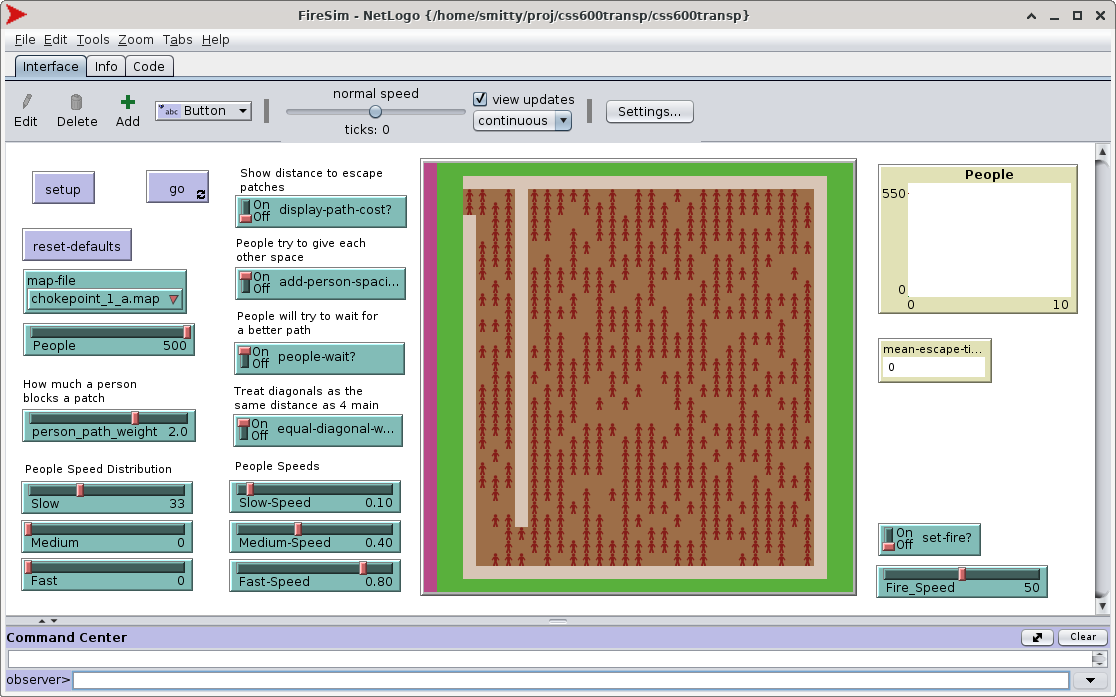
\includegraphics[width=.75\linewidth]{./figures/fire_sim_ui.png}
  \caption{Evac Sim UI implemented in NetLogo}
\end{figure}

One of the foundations of our simulation efforts was the ability to run experiments on a variety of maps, which mostly incrementally changed a key feature.  In order to accomplish this we implemented a custom map loader in NetLogo such that we could quickly develop custom layouts externally and procedurally load them at experiment time \ref{expEnv}.  The method of loading maps involves reading a file in line by  line which reflected a NetLogo list.  This list was then used to sequentially set the patch to the corresponding state, be it safety patch, grass, floor, or wall.  The code for loading a map is provided below.



\begin{lstlisting}[language=lisp, caption={Map loading procedure in NetLogo},captionpos=b, frame=single]
to load-map
  file-open map-file
  ; xdim and ydim are half the dimensions
  ; in width and height
  let row  ydim
  while [not file-at-end?]
  [
    ; read each line in	
    let linestr file-read-line
    ; load line into list variable
    let line read-from-string linestr
    let col  0 - xdim
    ; for each element in list set the patch color 
    ; to a value from a table of color mappings
    foreach line [      
      [x] ->
      ask patch col row [ 
            set pcolor table:get map_table x 
      ]
      set col (col + 1)
    ]
  set row (row - 1)
  ]
  file-close
end
\end{lstlisting}

Users may create map files in a separate text editor. Each cell reflects the desired patch state in the world, where 3 = safety, 0 = grass, 1 = floor, and 2 = wall. An important note is the beginning and ending brackets '[ ]'.  These are necessary for NetLogo to correctly load each line as a list structure from the line's string representation.  Below is an example portion of a map file.  

\begin{lstlisting}[language=lisp, caption={Example map file, 3 rows},captionpos=b, frame=single]
[3 0 0 2 2 2 2 2 2 2 2 2 2 2 2 2 2 2 2 2 2 2 2 2 2 0 0]
[3 0 0 1 1 1 1 2 1 1 1 1 1 1 1 1 1 1 1 1 1 1 1 1 2 0 0]
[3 0 0 2 1 1 1 2 1 1 1 1 2 1 1 1 1 1 2 1 1 1 1 1 2 0 0]
\end{lstlisting}

Since our map creation needs were constrained to the few experiments that we planned to execute we did not implement a procedural way to generate maps.  This functionality, while one of our stretch goals, had to be dropped in the interests of deadlines.  If one were to expand upon our work then there are number of mechanisms to generate layouts \cite{mirahmadiNovelAlgorithmRealtime2012} such that further experiments could be devised without the human intensive effort of generating maps by hand.  Such possibilities include evaluations of optimal floor plans through a guided search or ablative studies on the subtle modifications of ideal floor plans.

Our simulation grid world is governed by the patch type.  The safety patch (pink) is used as the foundation for our pathing algorithm described here \ref{move}.  The grass and floor patches (green and brown) are areas in which agents can  move freely.  The two different types of patches are not just for aesthetics but are a residual from original plans to implement a fire aspect which would have burnt differently on different patches.  The final patch type is the wall (light brown) which blocks agents from moving through.

The agent's themselves are also defined fairly simply.  They are principally defined by the speed at which they move, a value greater than 0 and less than 1.  They also have an internal counter for how long they have been on the map which is used to calculate the mean escape time.  This value increments on each global tick unless the agent has reached a safety patch.  In order to allow for ease of experimentation there are 3 groups of agents labeled slow, medium, and fast.  Despite the label semantics, each group can be assigned its own speed depending on the wishes of the experimenter.  During each movement step the agent moves the speed of the group that they are assigned to.  The experimenter can also set the number of agents in the environment from 0 to 500 before each simulation as expressed by the parameter $P$ below.  A helper function that we provide is the ability to maintain the ratio of numbers of slow, medium, and fast agents no matter the total number of agents.  This ratio is calculated in the following algorithm where $S$, $M$, and $F$ are the values specified by the experimenter in sliding values between 0 and 10.

\begin{equation}
\text{count of slow people} =\frac { S} {S + M + F} * P
\end{equation}

\subsection{Movement Mechanisms} \label{move}
In this section we will go over the mechanisms which dictate how our agents move throughout the environment.  Traditionally, in an environment where an agent is moving towards a goal, each agent's path to that goal will be calculated individually through the environment\footnote{http://www.cs.us.es/~fsancho/?e=131}.  In our situation we implemented a simplified pathing algorithm which instead calculates global weights for each environmental patch in which all agents flow to the lowest weight.  These weights grow in relation to their distance to the safety patches and as agents move over them by imparting their own weight to the patch.  This simplified pathing allows for much quicker computation of routes and therefor quicker executions of simulations for our experiments.

The following will provide an overview of how the weighting mechanisms work and the choices agents make on whether to move.  The foundation of movement is the weight of a given patch, or the cost as described below. The cost metric is defined as the distance from the patch to be considered $P$ and the nearest safety patch $P_s$.  While there may be many safety patches, for the sake of brevity, we assume that $P_s$ is resolved \emph{a priori} as the closest.  We can confidently declare this since the weighting implementation iteratively grows from each safety patch such that when it reaches a candidate patch it has been reached by the closest one.  This distance cost is also modified by the presence of an agent, $Agent(P)$, on that patch.  This agent's weight, $A_w$, is configurable by the user.  Of important note is that the weight is calculated independently of agents that may reside on patches between a patch and the safety patch.  This is the simplified pathing mechanism at work in that only local environment calculations are conducted.
\begin{align}
cost(P)  = distance(P_s, P) + Agent(P) * A_w \nonumber \\
Agent(P)=
\begin{cases}
1, & \text{Agent Present}  \\
0, & \text{Agent Not Present} 
\end{cases}
\end{align}

The distance measurement is not as simple as calculating the Euclidean distance.  Since our environment is a grid world that is inhabited by blocking obstacles we can only consider movement in either the 4 cardinal directions or the 8 neighboring directions.  These two options, which are additionally configurable by the user, determine how the distance between patches are measured.  The distance between 2 points $P_1$ \& $P_2$ is optionally defined by the flag $equal-diagonal-weight?$.  If false the distance is the Manhattan distance \footnote{ https://www.sciencedirect.com/topics/mathematics/manhattan-distance}. If true the distance is the Chebyshev distance \footnote{https://en.wikipedia.org/wiki/Chebyshev\_distance}. While this algorithm for distance works in an open world it doesn't account for the blocking obstacles.  This is another side effect of how the actual implementation works.  By growing outward from the safety patches and around obstacles the actual distance calculation is only ever considered for patches that are next to each other.  This makes our implementation a narrow case of the algorithm below in that all distances we calculate equal 1 and the real choice is how we choose the next patches as either the Manhattan or the Chebyshev neighborhood.
\begin{align}
distance(P_1, P_2)  = \nonumber\\
equal-diagonal-weight?=
\begin{cases}
	max(|x_1-x_2|, |y_1-y_2|), & True \\
	|x_1-x_2|+ |y_1-y_2|, & False
\end{cases}
\end{align}

Now that we have our patch weights to inform our movement decisions it is time to actually make the decision of where to move to.  For this choice we simply choose the neighbor patch that has the lowest cost, where the neighbors are defined as the 4 patches above, below, right, and left of our current patch.  Once we know which patch is lowest we take the vector at that patch and multiply it by our agent's speed.  So, for a given agent $A$ the vector to move is given by the vector of the lowest cost neighbor patch times our agent's speed. 


\begin{equation}
move(A) = V( min(cost(neighbors_4 (A_p))) ) * S_a
\end{equation}

\begin{align}
neighbors_4 (P)  = \{patch(P_x - 1, P_y -1), patch(P_x + 1, P_y -1), \nonumber \\ 
patch(P_x - 1, P_y + 1),patch(P_x + 1, P_y + 1)\}   
\end{align}


We have an additional parameter to account for situations where the cost of all neighboring patches is greater than the current patch. The flag $people-wait?$ allows simulators to decide whether or not to stay put and wait for a better patch or to always move even if the new patch has a higher cost.  This flag redefines the $move(A)$ function as $move(A)$ if the flag is false and if the cost of the current patch is less than $move(A)$ then to not move.
\begin{equation}
people-wait?=
\begin{cases}
min(cost(A_p), move(A)), & True \\
move(A), & False
\end{cases}
\end{equation}

Another phenomena we wished to capture is the ability for agent's to give each other space.  This is configurable through the $add-person-spacing?$ flag.  When the flag is true the cost of a patch is redefined to be the normal cost plus the sum of all the neighbors with agents times the agent's weight divided by 10.  This scaling factor of $1/10$ has been determined through trial and error and is something that could be exposed to user control in the future.  For ease of implementation and increased computation time the actual calculation is done from the perspective of the agent in that each agent has their scaled weight applied to its patch neighbors.

\begin{align}
add-person-spacing?= \nonumber  \\
\begin{cases}
	cost(P) + \sum Agent(neighbors_4(P)) * A_w / 10, & True \\
	cost(P), & False
\end{cases}
\end{align}

The grid world, while maybe too much of a simplification of real world dynamics, enables us to implement complex behaviors through simple straightforward algorithms.  These complex behaviors have enabled us to conduct a few interesting experiments described in the following sections.

\section{Experiments}

The range of experiments we have decided to conduct seeks to explore specific phenomena based on layouts \ref{expLayout}, agent settings \ref{expAgent}, and replicating human behavior \ref{emergentBehavior}.  In order to hone in on the most important features we have attempted to reduce each problem to its foundations through meticulous experiment design.  In order facilitate these experiments we developed a robust experimentation harness \ref{expEnv} to rapidly execute large and varied sets of experiments in NetLogo.  It is our goal to generate reference examples of easily understandable experiments that can help in exploring agent-based simulations in the NetLogo.  These experiments are designed to be the starting point for future and more complex evaluations of agent based evacuation models.


\subsection{Experimental Environment} \label{expEnv}
This section describes our experiment harness that we built using NetLogo's
Behavior Space functionality.  Behavior Space supports supplying simulation arguments via an XML document,
invoking the NetLogo engine via a script pointing to the XML, and then capturing
the results via the standard output.

This lends itself to scripting via Python \footnote{https://www.python.org/}. The goal had been to extract the
initial Behavior Space XML content directly from the .nlogo file, and then craft
a SQLAlchemy \footnote{https://www.sqlalchemy.org/} model on the fly that would support storing results in an RDBMS,
e.g. SQLite \footnote{https://sqlite.org/index.html}. That proved out of reach due to the advanced nature of SQLAlchemy,
so a hand-crafted model was used, which makes alterations to the underlying
model more maintenance intensive.  While we stored the results in a local SQLAlchemy file, a mere update to the
connection string would allow storing results in an enterprise RDBMS to good
effect.

Another Open Source tool that was used extensively was PyTest \footnote{https://docs.pytest.org/en/stable/}. Billed as a
unit testing framework, PyTest supports breaking the problem down into granular
fixtures and then combing them in a Lego-like fashion that lends itself to the
problem space. For example, while Behavior Space allows stepped alteration of
numerical parameters in a model, swapping out map file names is not directly
supported. Implementing a Python function to generate the map file names and
then re-writing the XML was far more convenient than having distinct
experiments for each map.

Generating parameters inputs via functions also supports enforcing invariants
across multiple ones, for example, the number of slow/medium/fast people. These
were three discrete integers, but were really percentage chunks of the people
variable.

SQLite proved really helpful when we discovered some scalability issues with
NetLogo itself. While there was no time to light off a Java debugger and delve
into the root cause, we saw decreasing ability of the system to complete the
ordered number of runs as the number of Agents increased and the distribution
shifted from slow to medium. It became useful to make a single SQLite file for
each increment of the people variable and then merge the results in a script
after the fact.

Finally, Python's data science facilities are well-known \footnote{https://www.scipy.org/index.html}, supporting arbitrary visualization pipelines.  Where visualizations were required to show results we leveraged the Matplotlib library to generate those graphs \footnote{ https://matplotlib.org/}.

\subsection{Experimental Parameters}
Need to talk about how agents are placed randomly throughout map, which is why we execute multiple runs.

need to break down the parameters and what they do.  

For the map files in use, there were 10 runs against the map files, capturing
mean-escape-time for the agents.

\begin{tabular}{ l | l }
VARIABLE & MEANING / VALUE \\
map-file & Name of map file to set up. \\
People & Number  of people. Held constant at 500. \\
person\_path\_weight & Agent blockage factor for patch \\
Slow & Percentage moving at this rate, which we set to 100 \\
Medium & Set to 0 \\
Fast & Set to 0 \\
Slow-Speed & 0.3 patches \\
Medium-Speed & 0.75 patches \\
Fast-Speed & 1.0 patches \\
add-person-spacing? & true \\
equal-diagonal-weight? & true \\
display-path-cost? & false \\
people-wait? & true \\
set-fire? & false \\
Fire\_Speed & 50 \\
mean-escape-time & output \\
\end{tabular}

\subsection{Experiments Based on Layouts} \label{expLayout}

The layout of an environment is probably the largest factor that determines evacuation behavior.  These layouts often have compounding features that work together to impact an evacuation\cite{abmEvac}. For our experiments based on the layouts we attempted to isolate those discreet features and exaggerate them such that the actual impact on evacuation can be seen.  These experiments build off of a base map showcasing that feature but replicating it with variations and plotting that impact on average evacuation time.


\subsubsection{Choke Point Experiment}

Our choke point experiments seek understand how choke points impact evacuation.  For our purposes a choke point is a narrowing of the map that people must travel through.  This is a subset of the often used definition of a choke point as a critical point at which people must move through\cite{evacOptions}.  We begin our map design with a map with one choke point close to the exit.  We expand upon this by adding more choke points to that map as well as starting new lines of maps that have their choke point start further away from the exit.

\begin{figure*}[!ht]
  \centering
  \begin{minipage}[b]{\linewidth}
    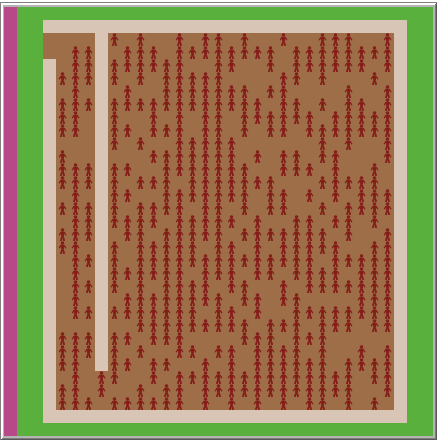
\includegraphics[width=0.15\textwidth]{./figures/chokepoint_1_a.png}
    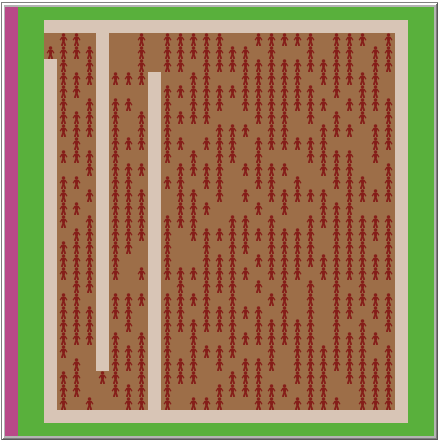
\includegraphics[width=0.15\textwidth]{./figures/chokepoint_1_b.png}
    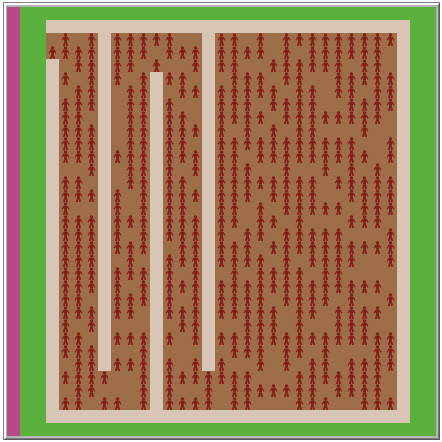
\includegraphics[width=0.15\textwidth]{./figures/chokepoint_1_c.png}
    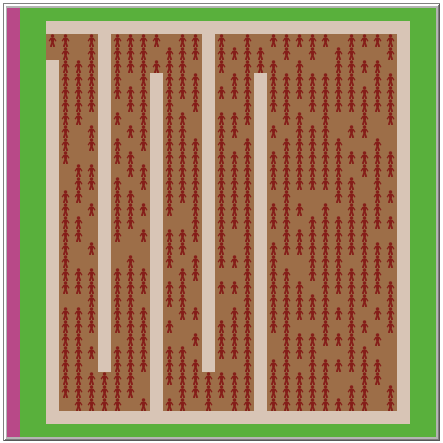
\includegraphics[width=0.15\textwidth]{./figures/chokepoint_1_d.png}
    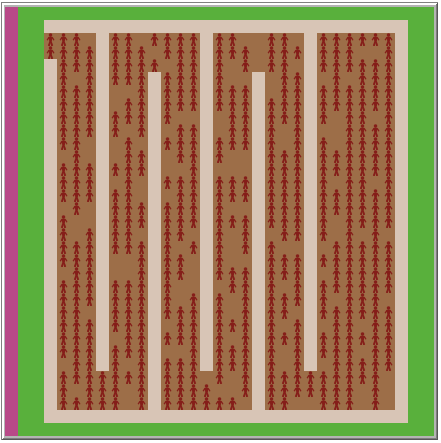
\includegraphics[width=0.15\textwidth]{./figures/chokepoint_1_e.png}
    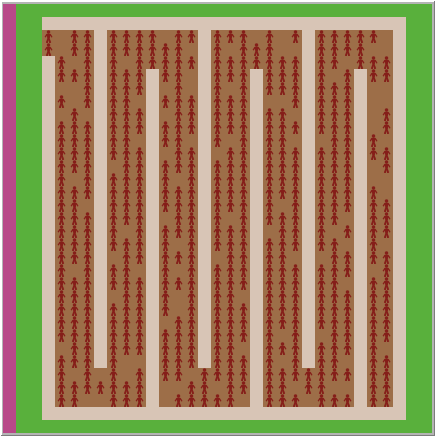
\includegraphics[width=0.15\textwidth]{./figures/chokepoint_1_f.png}
  \end{minipage}
  \begin{minipage}[b]{\linewidth}
    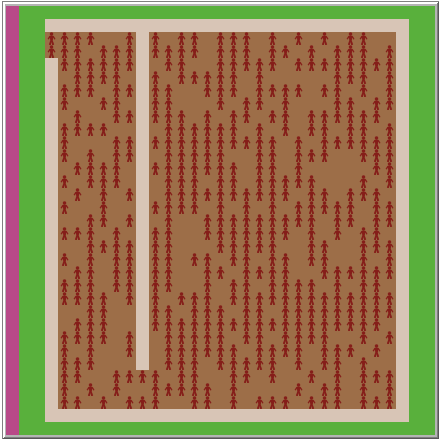
\includegraphics[width=0.15\textwidth]{./figures/chokepoint_2_a.png}
    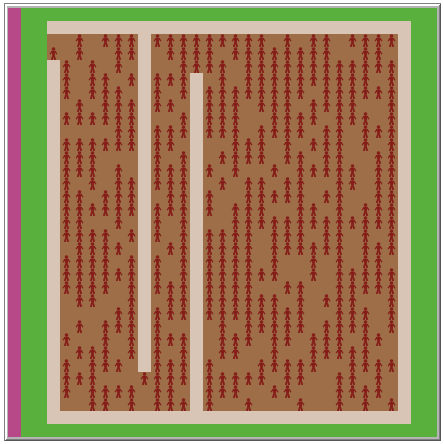
\includegraphics[width=0.15\textwidth]{./figures/chokepoint_2_b.png}
    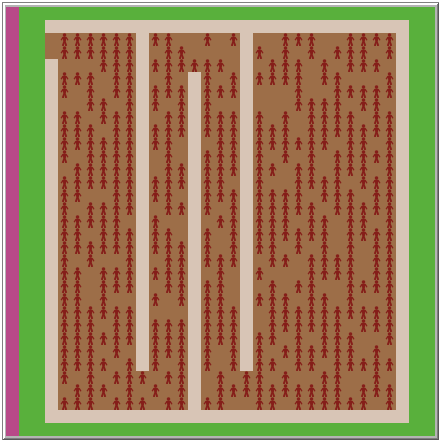
\includegraphics[width=0.15\textwidth]{./figures/chokepoint_2_c.png}
    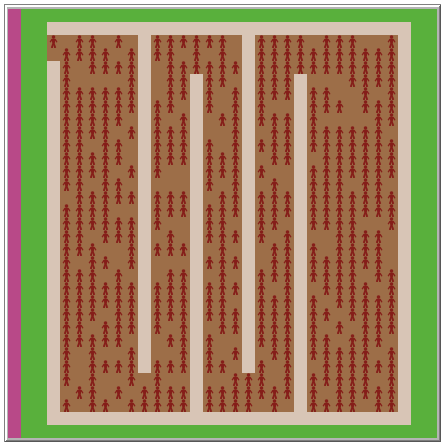
\includegraphics[width=0.15\textwidth]{./figures/chokepoint_2_d.png}
    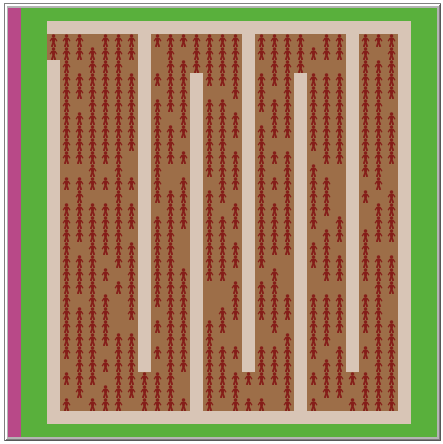
\includegraphics[width=0.15\textwidth]{./figures/chokepoint_2_e.png}
  \end{minipage}
  \begin{minipage}[b]{\linewidth}
    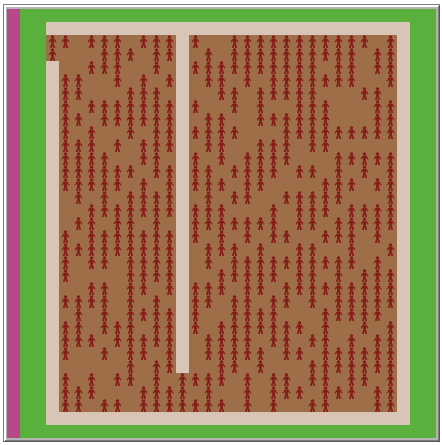
\includegraphics[width=0.15\textwidth]{./figures/chokepoint_3_a.png}
    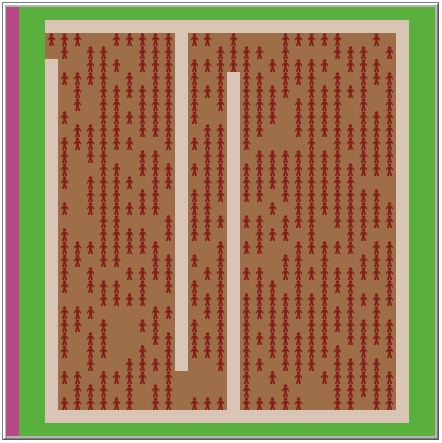
\includegraphics[width=0.15\textwidth]{./figures/chokepoint_3_b.png}
    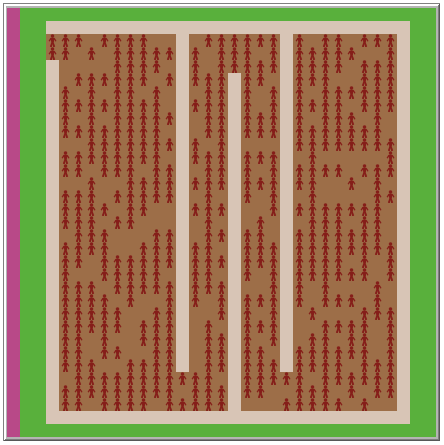
\includegraphics[width=0.15\textwidth]{./figures/chokepoint_3_c.png}
    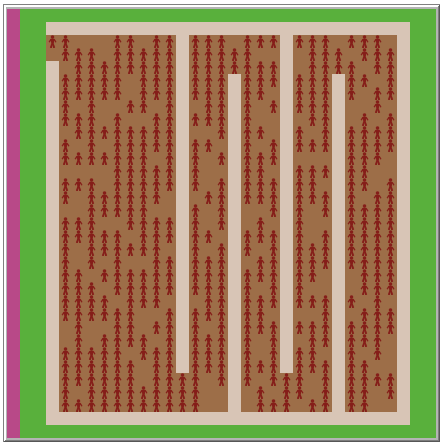
\includegraphics[width=0.15\textwidth]{./figures/chokepoint_3_d.png}
  \end{minipage}
  \caption{Choke point maps}
\end{figure*}

For each map we executed a number of runs and captured the mean escape time, with results stated below \ref{fig:chokepointResults}.  By increasing the number of choke points we sought to understand the initial impact of a choke point as well as the impact of sequential additions which we expected to have decreasing impact. The intuition behind this is that even with more choke points agents will start to align to the most narrow width.  We also increased the distance from the final choke point to the exit to evaluate if the ability to spread back out can negate some of the negatives of the choke point.  

\subsubsection{Exit Dimensions}

Our next layout based experiment evaluates how exit dimension size and place impacts evacuation speeds.  We varied the size of the exits as well as their placements alternating between states of one exit on one side, exit evenly split to opposite sides, and exit evenly split into 1 width wide exits all on one side.  As shown below, each column of maps has the same overall exit size while each row shows the various placement strategies.

\begin{figure*}[!ht]
  \centering
  \begin{minipage}[b]{.75\linewidth}
    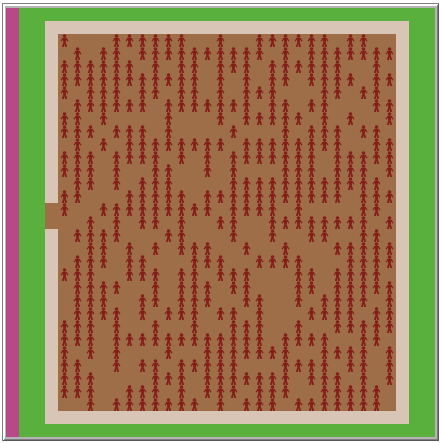
\includegraphics[width=0.24\textwidth]{./figures/exit_dims_2_a.png}
    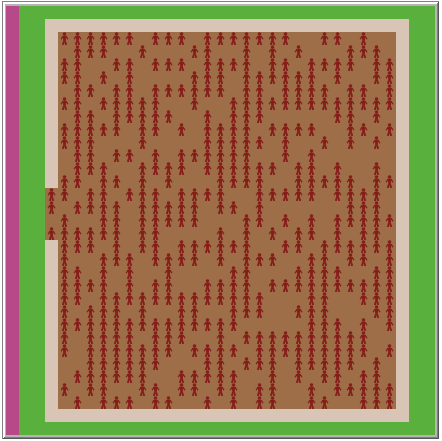
\includegraphics[width=0.24\textwidth]{./figures/exit_dims_4_a.png}
    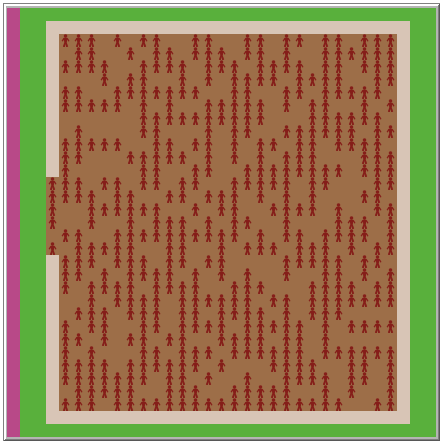
\includegraphics[width=0.24\textwidth]{./figures/exit_dims_6_a.png}
    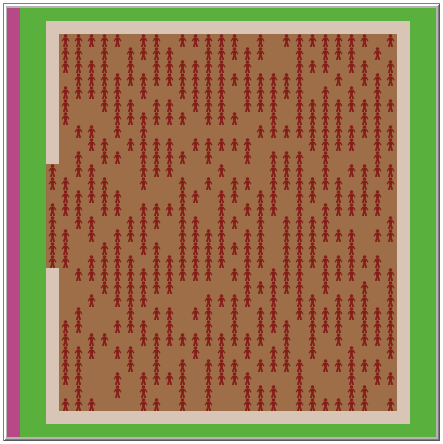
\includegraphics[width=0.24\textwidth]{./figures/exit_dims_8_a.png}
  \end{minipage}
  \begin{minipage}[b]{.75\linewidth}
    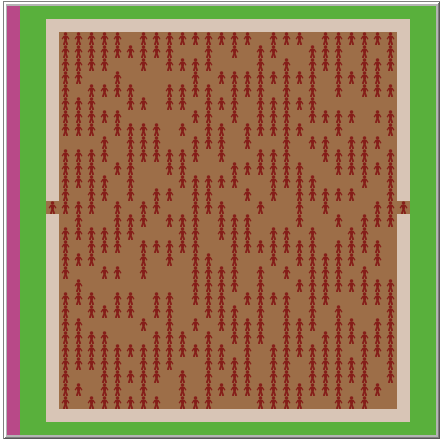
\includegraphics[width=0.24\textwidth]{./figures/exit_dims_2_b.png}
    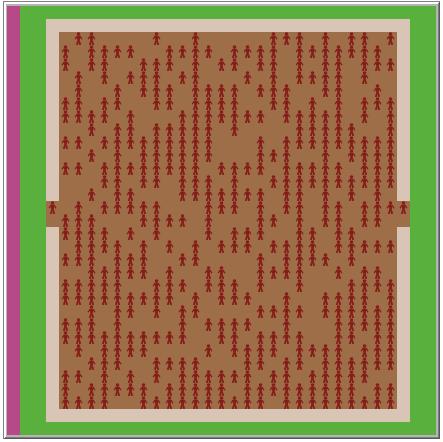
\includegraphics[width=0.24\textwidth]{./figures/exit_dims_4_b.png}
    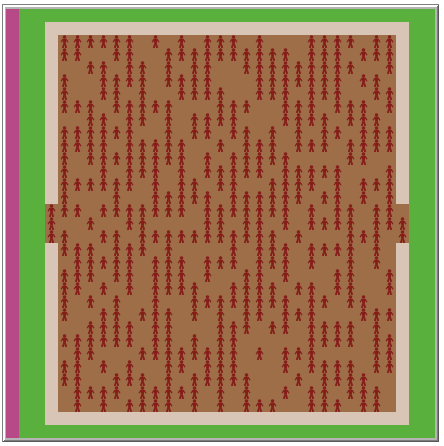
\includegraphics[width=0.24\textwidth]{./figures/exit_dims_6_b.png}
    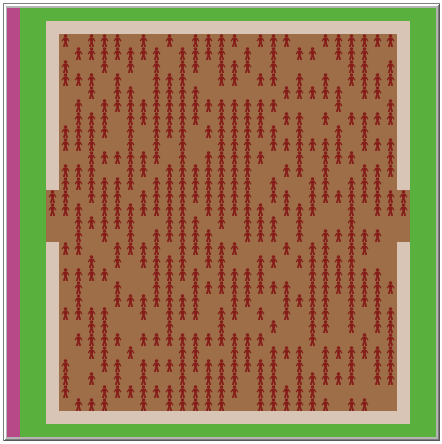
\includegraphics[width=0.24\textwidth]{./figures/exit_dims_8_b.png}
  \end{minipage}
  \begin{minipage}[b]{.75\linewidth}
    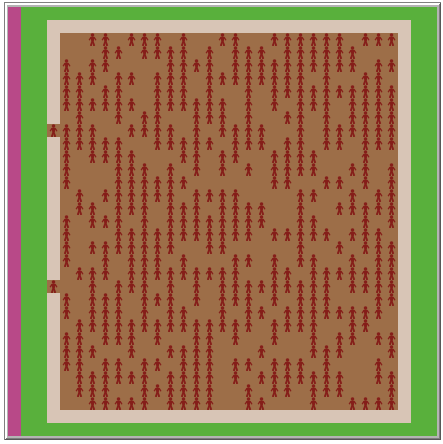
\includegraphics[width=0.24\textwidth]{./figures/exit_dims_2_c.png}
    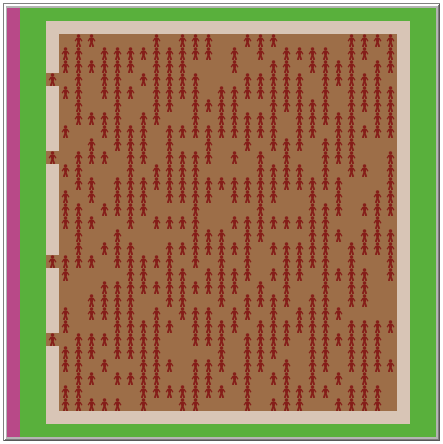
\includegraphics[width=0.24\textwidth]{./figures/exit_dims_4_c.png}
    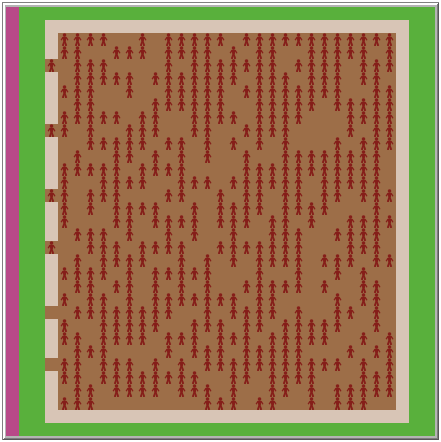
\includegraphics[width=0.24\textwidth]{./figures/exit_dims_6_c.png}
    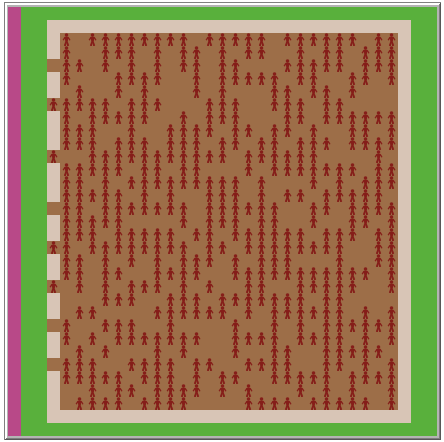
\includegraphics[width=0.24\textwidth]{./figures/exit_dims_8_c.png}
  \end{minipage}

  \caption{Exit Dimensions Maps}
\end{figure*}

Similar to the choke points experiment, we captured the mean escape time for a number of runs on each map, with the results provided below \ref{fig:exitdimsResults}.  In these experiments we hoped to gain some insight, when dimensions are held the same, can exit placements be beneficial to escaping pedestrians.  This is why the map itself is an empty room, so that the only layout impact we have is the size and placement of the exits.

\subsection{Experiments Based on Agent Features} \label{expAgent}

Experiments based on agent features explore how the properties of pedestrians affect escape times.  These properties maybe simple measures of speed of movement to complex behaviors such as knowledge of the layout.  In general, for all of our experiments, all agents have knowledge of the complete layout as derived from our global pathing algorithm which impacts each agent the same.  For our specific experiment we evaluated how speed distribution between agents impacts the escape times.  

The goal of varying the distribution of speeds among the agents is to see if that people moving at different speeds introduces a negative factor, \emph{a la} a turbulence similar to fluid dynamics.  While we expect the average escape time to decrease while we move from more slow agents to faster agents, we are looking for a deviation from that expected decrease as shown below \ref{fig:speedResults}.  If various movement speed distributions do introduce this turbulence into the system we can begin further discussions and experiments on how to mitigate these impacts through more efficient designs.


\subsection{Experiments Replicating Emergent Crowd Behaviors} \label{emergentBehavior}
- mainly from this paper \cite{almeidaCrowdSimulationModeling2013}  .  This section will cover how we hope to see these emergent behaviors in our environments even though we use a simplified pathing strategy.  This could lead to simpler models with less resource requirements.



\begin{figure}[!htbp]
  \centering
  \subfloat[Evacuation with no herding ]{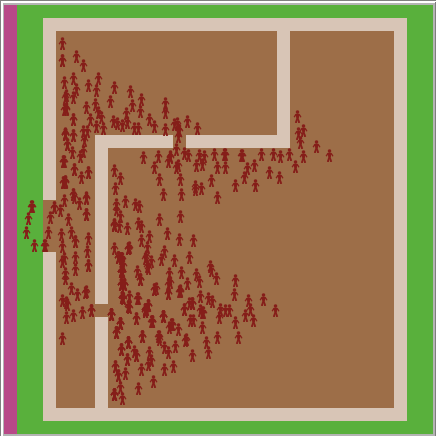
\includegraphics[width=0.4\textwidth]{./figures/Herding1.png}\label{fig:f1}}
  \hfill
  \subfloat[Evacuation with herding (i.e. ignoring viable exit)]{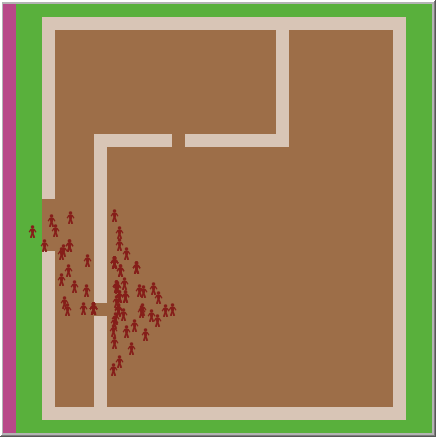
\includegraphics[width=0.4\textwidth]{./figures/Herding-2.png}\label{fig:f2}}
  \caption{Herding behavior replicated through residual escape pathing from agents that never considered the alternative route.}
\end{figure}

\begin{figure}[!htbp]
  \centering
  \subfloat[No clogging due to people not blocking paths ]{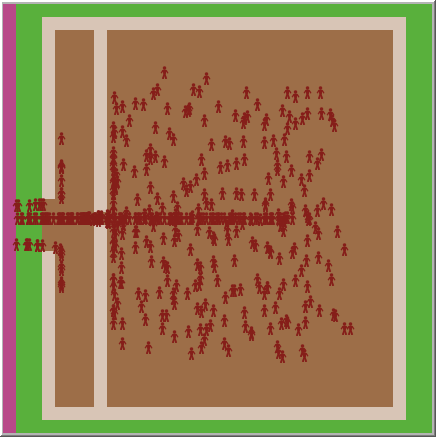
\includegraphics[width=0.4\textwidth]{./figures/clogging1_clean.png}\label{fig:f1}}
  \hfill
  \subfloat[Clogging due to increased weight per person on a patch]{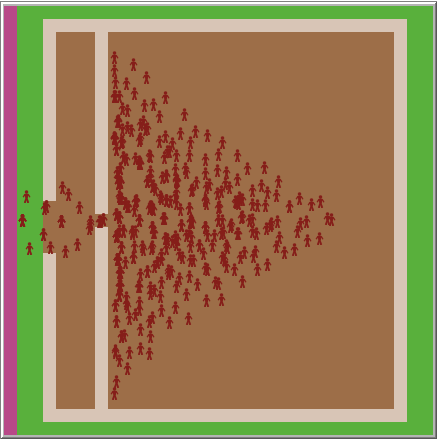
\includegraphics[width=0.4\textwidth]{./figures/clogging2_clean.png}\label{fig:f2}}
  \caption{Clogging behavior replicated through a weight attribute calculated for each patch an agent is on as well as a configurable additional weight for each agent's neighboring patch. }
\end{figure}


if we can show that we achieve similar results even though we use a simplified pathing algorithm and abm environment i think that would be insightful



\section{Results}

The results showed that adding more length to the chokepoint pipeline did not
result in a linear increase in the exit time. Rather, the Actors resembled a
fluid dynamics problem, reaching a uniform flow and making good their escape.

More exits is better, especially if not on the same side, but there is not a
linear increase with additional exits.

\begin{figure} 
  \centering
  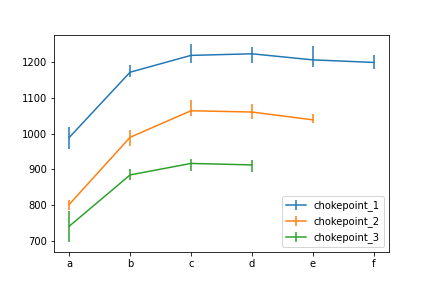
\includegraphics[width=.9\linewidth]{./figures/chokepoint_graph.png}
  \caption{Choke point results}
  \label{fig:chokepointResults}
\end{figure}
\begin{figure}
  \centering
  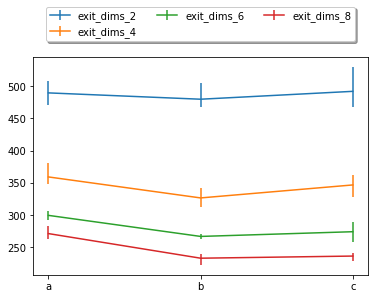
\includegraphics[width=.75\linewidth]{./figures/exit_dims_graph.png}
  \caption{Exit dimensions results}
  \label{fig:exitdimsResults}
\end{figure}

\begin{figure}
  \centering
  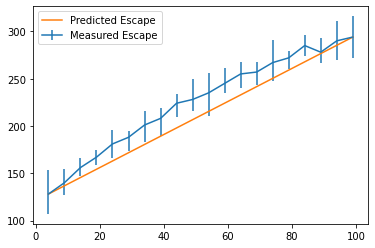
\includegraphics[width=.75\linewidth]{./figures/speed_dist_test.png}
  \caption{Agent speed distribution results}
  \label{fig:speedResults}
\end{figure}

chokepoint1
\begin{tabular}{ r | r | r | r | r }
map & MIN  & AVG    & MAX    & VAR    \\
a &  966.4 & 1006.0 &  963.0 &  995.6 \\
b & 1155.6 & 1190.0 & 1149.0 & 1181.6 \\
c & 1207.0 & 1243.0 & 1198.0 & 1234.9 \\
d & 1217.5 & 1234.0 & 1210.0 & 1231.1 \\
e & 1202.4 & 1243.0 & 1200.0 & 1226.0 \\
f & 1183.1 & 1212.0 & 1179.0 & 1206.3 \\
\end{tabular}
\\
\\
chokepoint2
\begin{tabular}{ r | r | r | r | r }
map & MIN  & AVG    & MAX    & VAR    \\
a &  790.8 &  833.0 &  781.0 &  819.8 \\
b &  975.7 & 1025.0 &  970.0 & 1015.7 \\
c & 1036.3 & 1071.0 & 1017.0 & 1071.5 \\
d &  103 9.3 & 10710 & 134.0 & 165.5 \\
e & 10 34. 8 & 1055.0& 102.0 & 105.2 \\  
\end{tabular}
\\
\\
chokepoint3
\begin{tabular}{ r | r | r | r | r }
map &  MIN   & AVG   & MAX   & VAR   \\
a   &  717.6 & 758.0 & 704.0 & 751.9 \\
b   &  886.9 & 919.0 & 880.0 & 911.2 \\
c   &  905.2 & 952.0 & 900.0 & 937.3 \\
d   &  902.3 & 925.0 & 894.0 & 919.2 \\
\end{tabular}          
\\  
\\
extdims2
\begin{tabular}{ r | r | r | r | r }
map & MIN   & AVG   & MAX   & VAR   \\
a   & 480.6 & 516.0 & 472.0 & 502.5 \\
b   & 482.9 & 522.0 & 474.0 & 510.0 \\
c   & 481.3 & 524.0 & 473.0 & 510.6 \\
\end{tabular}                          
\\
\\
exitdims4
\begin{tabular}{ r | r | r | r | r }
map & MIN   & AVG   & MAX   & VAR   \\
a   & 348.4 & 368.0 & 342.0 & 367.3 \\
b   & 319.2 & 344.0 & 317.0 & 336.3 \\
c   & 334.3 & 365.0 & 328.0 & 358.8 \\
\end{tabular}
\\
\\
exitdims6
\begin{tabular}{ r | r | r | r | r }
map & MIN   & AVG   & MAX   & VAR   \\
a   & 292.0 & 302.0 & 287.0 & 301.7 \\    
b   & 262.0 & 285.0 & 258.0 & 277.9 \\
c   & 265.8 & 290.0 & 265.0 & 280.3 \\
\end{tabular}
\\
\\
exitdims8
\begin{tabular}{ r | r | r | r | r }
map &  MIN   &  AVG  & MAX   & VAR   \\
a   &  264.7 & 279.0 & 263.0 & 276.2 \\
b   &  230.4 & 243.0 & 228.0 & 240.3 \\
c   &  231.4 & 250.0 & 231.0 & 242.7 \\
\end{tabular}  
\\
\\
chokepoint.map, 100 people, variance=17161
\begin{tabular}{ r | r | r | r | r }
slow & medium & MIN   & AVG   & MAX \\
   4 & 96     & 107.0 & 128.0 & 153.0 \\
   9 & 91     & 127.0 & 140.0 & 154.0 \\
  14 & 86     & 147.0 & 156.0 & 166.0 \\
  19 & 81     & 159.0 & 167.0 & 175.0 \\
  24 & 76     & 166.0 & 181.0 & 196.0 \\
  29 & 71     & 174.0 & 188.0 & 195.0 \\
  34 & 66     & 183.0 & 201.0 & 216.0 \\
  39 & 61     & 189.0 & 208.0 & 219.0 \\
  44 & 56     & 209.0 & 224.0 & 234.0 \\
  49 & 51     & 216.0 & 228.0 & 250.0 \\
  54 & 46     & 210.0 & 235.0 & 256.0 \\
  59 & 41     & 235.0 & 245.0 & 261.0 \\
  64 & 36     & 240.0 & 255.0 & 268.0 \\
  69 & 31     & 243.0 & 257.0 & 268.0 \\
  74 & 26     & 248.0 & 267.0 & 291.0 \\
  79 & 21     & 260.0 & 272.0 & 279.0 \\
  84 & 16     & 274.0 & 285.0 & 296.0 \\
  89 & 11     & 267.0 & 278.0 & 293.0 \\
  94 &  6     & 270.0 & 290.0 & 311.0 \\
  99 &  1     & 272.0 & 294.0 & 316.0 \\
\end{tabular}  
%
%200,34,66,0,0.3,1.0,0.75,269.0,292.0,317.0,29232.0
%200,39,61,0,0.3,1.0,0.75,291.0,309.0,330.0,29232.0
%200,44,56,0,0.3,1.0,0.75,300.0,318.0,334.0,29232.0
%200,49,51,0,0.3,1.0,0.75,309.0,327.0,343.0,29232.0
%200,54,46,0,0.3,1.0,0.75,330.0,350.0,363.0,29232.0
%200,59,41,0,0.3,1.0,0.75,336.0,357.0,374.0,29232.0
%200,64,36,0,0.3,1.0,0.75,357.0,369.0,394.0,29232.0
%200,69,31,0,0.3,1.0,0.75,356.0,375.0,398.0,29232.0
%200,74,26,0,0.3,1.0,0.75,347.0,384.0,417.0,29232.0
%200,79,21,0,0.3,1.0,0.75,368.0,390.0,415.0,29232.0
%200,84,16,0,0.3,1.0,0.75,379.0,398.0,422.0,29232.0
%200,89,11,0,0.3,1.0,0.75,367.0,401.0,433.0,29232.0
%200,94,6,0,0.3,1.0,0.75,378.0,408.0,448.0,29232.0
%200,99,1,0,0.3,1.0,0.75,391.0,430.0,463.0,29232.0
%
%\\
%\\
%300,39,61,0,0.3,1.0,0.75,357.0,379.0,402.0,39602.0
%300,44,56,0,0.3,1.0,0.75,379.0,401.0,426.0,39602.0
%300,49,51,0,0.3,1.0,0.75,387.0,413.0,439.0,39602.0
%300,54,46,0,0.3,1.0,0.75,395.0,429.0,468.0,39602.0
%300,59,41,0,0.3,1.0,0.75,382.0,431.0,466.0,39602.0
%300,64,36,0,0.3,1.0,0.75,421.0,450.0,477.0,39602.0
%300,69,31,0,0.3,1.0,0.75,427.0,465.0,495.0,39602.0
%300,74,26,0,0.3,1.0,0.75,442.0,473.0,500.0,39602.0
%300,79,21,0,0.3,1.0,0.75,468.0,490.0,513.0,39602.0
%300,84,16,0,0.3,1.0,0.75,466.0,491.0,509.0,39602.0
%300,89,11,0,0.3,1.0,0.75,468.0,502.0,553.0,39602.0
%300,94,6,0,0.3,1.0,0.75,506.0,521.0,541.0,39602.0
%300,99,1,0,0.3,1.0,0.75,490.0,509.0,529.0,39602.0
%
%\\
%\\
%400,49,51,0,0.3,1.0,0.75,473.0,501.0,533.0,45878.0
%400,54,46,0,0.3,1.0,0.75,465.0,511.0,544.0,45878.0
%400,59,41,0,0.3,1.0,0.75,491.0,528.0,573.0,45878.0
%400,64,36,0,0.3,1.0,0.75,511.0,546.0,575.0,45878.0
%400,69,31,0,0.3,1.0,0.75,534.0,559.0,583.0,45878.0
%400,74,26,0,0.3,1.0,0.75,520.0,546.0,562.0,45878.0
%400,79,21,0,0.3,1.0,0.75,543.0,573.0,612.0,45878.0
%400,84,16,0,0.3,1.0,0.75,567.0,591.0,605.0,45878.0
%400,89,11,0,0.3,1.0,0.75,557.0,589.0,617.0,45878.0
%400,94,6,0,0.3,1.0,0.75,566.0,592.0,623.0,45878.0
%400,99,1,0,0.3,1.0,0.75,554.0,591.0,640.0,45878.0
%
%\\
%\\
%500,49,51,0,0.3,1.0,0.75,543.0,575.0,637.0,54139.0
%500,54,46,0,0.3,1.0,0.75,535.0,571.0,610.0,54139.0
%500,59,41,0,0.3,1.0,0.75,540.0,594.0,620.0,54139.0
%500,64,36,0,0.3,1.0,0.75,558.0,606.0,638.0,54139.0
%500,69,31,0,0.3,1.0,0.75,591.0,622.0,655.0,54139.0
%500,74,26,0,0.3,1.0,0.75,615.0,646.0,680.0,54139.0
%500,79,21,0,0.3,1.0,0.75,609.0,642.0,674.0,54139.0
%500,84,16,0,0.3,1.0,0.75,611.0,655.0,700.0,54139.0
%500,89,11,0,0.3,1.0,0.75,633.0,684.0,709.0,54139.0
%500,94,6,0,0.3,1.0,0.75,644.0,679.0,713.0,54139.0
%500,99,1,0,0.3,1.0,0.75,648.0,674.0,723.0,54139.0
\section{Future Work}
Here we can expand on improvements we would make, additional features we could add (smoke multi-floor etc.), additional experiments, and porting to other environments

Add procedurally generated maps as mentioned in \ref{Environment}

add multilevel or 3d component

add smoke and fire spread

port to mason \footnote{https://cs.gmu.edu/~eclab/projects/mason/} or Mesa \footnote{https://mesa.readthedocs.io/en/master/tutorials/intro\_tutorial.html}

\section {Conclusion}

The simpler the layout, with more and diversified exit options, the more optimal
the evacuation results.


\bibliographystyle{plain}
\bibliography{css600}

\end{document}
